\chapter{Digitālo prasmju ietekmes analīze uz darba tirgu}
\paragraph{}
Mūsdienu pasaule strauj attīstās un ar vien vairāk tiek runātas par dažādu arodu izzušanu.
Taču veidojās arī jaunie darba veidi, ar vien vairāk šie jaunie arodi prasa cilvēkam zināt
jaunās tehnoloģijas, datorprasmi gan pamatprasmju līmenī, gan padziļināti.
Autors veic izpēti par Latvijas rādītājiem Eiropas Savienības līmenī izmantojot \acrlong{desi} 
(turpmāk tekstā \acrshort{desi}), kā arī šie rādītāji ir salīdzināti ar Latvijas tuvākiem kaimiņiem,
proti, Lietuvu un Igauniju.Otra datu grupa nāk no Latvijas atvērtās datu kopas, pievēršot plašāku 
uzmanību izglītībai un nodarbinātībai ITK jomai. Šī datu izpēte nepieciešama, lai varētu pieņemt 
labāku lēmumu par uzņēmuma Accenture Latvijas filiāle turpmāko sadarbību izglītības sektorā.
\paragraph{}
Accenture Latvia par savu korperatīvo sociālo atbildību ir izvirzījusi tieši attīstību. Tam par pamatu nāk lielā nepieciešamība
pēc augsti kvalificētā darba spēka. Uzņēmums jau vairāk nekā 15 gadus veiksmīgi darbojas Latvijas teritorijā, taču asi izjūt
darba spēka trūkumu. Ieguldījums izglītībā palīdz labot situāciju, kā arī uzlabo Latvijas kopējo konkurētspēju Eiropā un pasaulē.
\section{Digitālās ekonomikas un savienojamības indeks}
%example plot
\textit{The \LaTeX\ Companion} book \cite{latexcompanion}
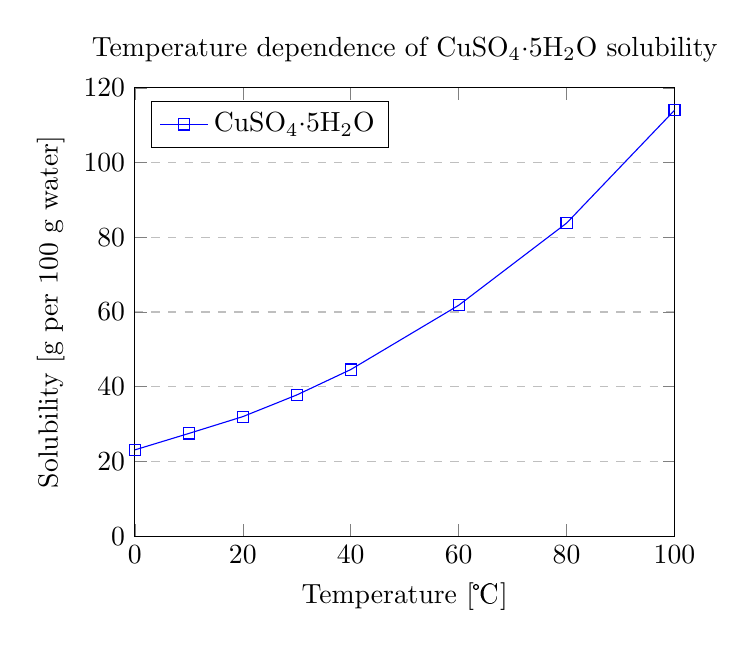
\begin{tikzpicture}
    \begin{axis}[
        title={Temperature dependence of CuSO$_4\cdot$5H$_2$O solubility},
        xlabel={Temperature [\textcelsius]},
        ylabel={Solubility [g per 100 g water]},
        xmin=0, xmax=100,
        ymin=0, ymax=120,
        xtick={0,20,40,60,80,100},
        ytick={0,20,40,60,80,100,120},
        legend pos=north west,
        ymajorgrids=true,
        grid style=dashed,
    ]
     
    \addplot[
        color=blue,
        mark=square,
        ]
        coordinates {
        (0,23.1)(10,27.5)(20,32)(30,37.8)(40,44.6)(60,61.8)(80,83.8)(100,114)
        };
        \legend{CuSO$_4\cdot$5H$_2$O}
     
    \end{axis}
\end{tikzpicture}
    \subsection{Savienojamība}
\begin{figure}[h]
    \label{att:desi_savienojamiba}
    \caption{DESI rādītāji}
    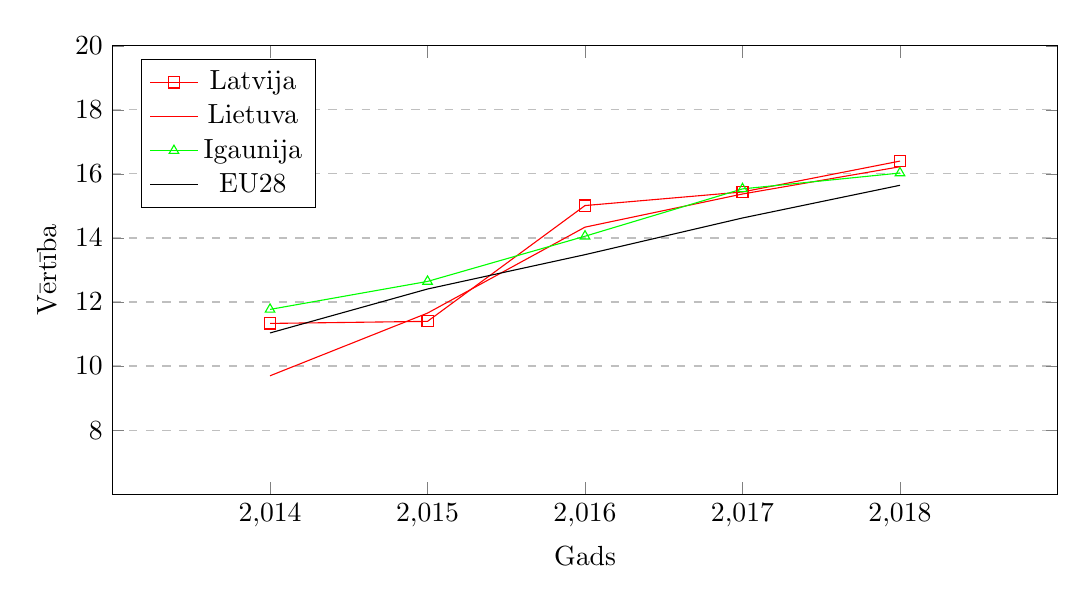
\begin{tikzpicture}
        \begin{axis}[
            x=2cm,
            xlabel={Gads},
            ylabel={Vērtība},
            xmin=2013, xmax=2019,
            ymin=6, ymax=20,
            xtick={2014,2015,2016,2017,2018},
            ytick={8,10,12,14,16,18,20},
            legend pos=north west,
            ymajorgrids=true,
            grid style=dashed,
        ]
        \addplot[
            color=red, 
            mark=square
            ]
            coordinates {
                (2014,11.3305)(2015,11.3951)(2016,15.0115)(2017,15.4357)(2018,16.4)
            };
        \addplot[
            color=red, 
            mark=circle
            ]
            coordinates {
                (2014,9.6959)(2015,11.6532)(2016,14.3374)(2017,15.3726)(2018,16.2237)
            };
        \addplot[
            color=green, 
            mark=triangle
            ]
            coordinates {
                (2014,11.7685)(2015,12.6421)(2016,14.0537)(2017,15.5321)(2018,16.0279)
            };
        \addplot[
            color=black, 
            mark=dot
            ]
            coordinates {
                (2014,11.0332)(2015,12.4053)(2016,13.478)(2017,14.6234)(2018,15.6445)
            };
        \legend{Latvija, Lietuva, Igaunija, EU28}
        \end{axis}
    \end{tikzpicture}
\end{figure}
\paragraph{}
2017. gadā Latvijai izdevās panākt diezgan lielu progresu kopējā savienojamības
aspektā, un tās izaugsmes temps līdzinājās ES vidējam. Attiecībā uz mājsaimniecību
fiksētās platjoslas pārklājumu valstī vērojama stagnācija – tā joprojām atpaliek no ES
vidējā rādītāja, ar 93\% mājsaimniecību pārklājumu Latvijai atrodoties 24. vietā.
Jāuzsver, ka gandrīz viss pārklājums nodrošina nākamās paaudzes piekļuvi (NPP)
(91\% mājsaimniecību) un pat ātrdarbīgo platjoslu (88\% mājsaimniecību), tādējādi
Latviju ierindojot starp vadošajām dalībvalstīm, kuru rādītāji krietni pārsniedz ES
vidējo. Arī 4G pārklājums Latvijā ir ļoti augsts (98\% mājsaimniecību). Ātrdarbīgās un
īpaši ātrdarbīgās platjoslas izmantošanas līmenis arī ir ievērojami augstāks par ES
vidējo: 42\% un 35\% mājokļu abonē ātrdarbīgas un īpaši ātrdarbīgas platjoslas
pakalpojumus, kas attiecīgi Eiropas Savienībā vidēji ir 33\% un 15,4\%. Tomēr,
neskatoties uz nelielu pieaugumu 2017. gadā, kopējā fiksētās platjoslas izmantošana
Latvijā vēl aizvien ir mazliet zem ES vidējā rādītāja. Šo tendenci zināmā mērā 
Digitālās ekonomikas un sabiedrības indekss 2018, ziņojums par Latviju. lpp. 4 no 11
kompensē daudz straujākais mobilās platjoslas pieslēgumu pieaugums, jo ir plašas
iespējas izvēlēties datu plānus par pieejamām cenām.
\paragraph{}
“Vidējās jūdzes projekts”, kas tika sākts 2012. gadā un kam piešķirts līdzfinansējums
no ES struktūrfondiem, lai lauku teritorijas savienotu ar valsts pamatinfrastruktūru,
tagad nonācis otrajā posmā. Plānots, ka otrā posma būvdarbi sāksies 2018. gada
pavasarī. Galvenokārt tie tiks veikti atlikušajās “baltajās” teritorijās (2014.–2015. gadā
apzināta 221 teritorija). Paredzēts, ka līdz 2020. gadam optiskie kabeļi tiks ierīkoti
2800 km garumā un izveidoti aptuveni 220 optiskā tīkla piekļuves punkti. Pēc tam
telesakaru operatoriem, izmantojot jauno tīklu, kas ļaus galalietotājiem piedāvāt
mazumtirdzniecības pakalpojumus, būs iespēja izveidot vietējās sakaru līnijas ar datu
pārraides ātrumu vismaz 30 Mbit/s (“pēdējā jūdze”). Tomēr šķiet, ka ne visur tiek
veiktas privātās investīcijas “pēdējās jūdzes” infrastruktūras izbūvē. Ir vajadzīgi
turpmāki centieni, piemēram, papildu valsts atbalsta shēmas un regulatīvi pasākumi,
lai novērtētu situāciju un piedāvātu risinājumus, kas attiecīgajos gadījumos ļautu
novērst ar “pēdējo jūdzi” saistīto plaisu. Iespēja mājās, pieslēdzoties no mobilajām
ierīcēm, izmantot mobilo operatoru nodrošinātos fiksētos sakaru pakalpojumus,
palīdz pārvarēt šo plaisu atsevišķos lauku apvidos, kur netiek veiktas investīcijas
“pēdējās jūdzes” savienojumos\cite{platjosla}
\paragraph{}
Optiskā tīkla izveidē un 4G pakalpojumu ieviešanā Latvija ir izvirzījusies starp
līderiem. Tomēr joprojām problemātiska ir digitālā plaisa, kas izveidojusies starp
pilsētu un laukiem. Lai to novērstu, praktisku labumu var sniegt nesen pieņemtie
noteikumi, ar kuriem tiek transponēta Platjoslas izmaksu samazināšanas direktīva.
Turklāt, lai nākotnē neatpaliktu no straujās savienojamības attīstības, visiem tirgus
dalībniekiem jābūt savlaicīgi pieejamiem piemērotiem spektra blokiem agrīnai 5G
tīkla izmēģināšanai un izvēršanai.

    \paragraph{}
Cilvēkkapitāla aspektā Latvija atpaliek no ES vidējās vērtības, un pēdējā gadā progress nav
panākts. Interneta lietotāju īpatsvars iedzīvotāju vidū gandrīz atbilst ES vidējam rādītājam,
tomēr 52 \% Latvijas iedzīvotāju joprojām trūkst digitālo pamatprasmju, kas tiem liedz efektīvi
lietot internetu, turklāt 19 \% digitālo prasmju vispār nav (par 2 punktiem vairāk nekā ES
vidējais rādītājs).
\paragraph{}
Latvijā digitālo prasmju līmenis sieviešu vidū ir nedaudz augstāks nekā vīriešiem. Sieviešu
vidū vismaz 50 \% ir digitālās pamatprasmes, taču vīriešiem tie ir tikai 46 \%. Atšķirīgs ir arī
strādājošo un nestrādājošo iedzīvotāju digitālo prasmju līmenis. No strādājošajiem 57 \%
digitālās prasmes ir pamata vai augstākā līmenī, savukārt nestrādājošo vidū šis rādītājs ir
tikai 33 \%. Arī izglītības līmenis ir svarīgs faktors saistībā ar digitālo prasmju apguvi. No tiem,
kas ieguvuši augstāko izglītību, 76 \% ir vismaz digitālās pamatprasmes (ES līmenī tie ir
84 \%), taču pamatizglītību vai vidēja līmeņa izglītību ieguvušo vidū šis īpatsvars ir tikai 35 \%.
Mazizglītotiem cilvēkiem šis rādītājs ir par 5 \% augstāks nekā ES vidējais, savukārt vidēji
izglītotiem cilvēkiem šī starpība salīdzinājumā ar ES vidējo rādītāju ir 20 punkti. IKT
speciālistu skaits ir stabils, taču ievērojami zem ES vidējā līmeņa. Turklāt pēdējos gados ir
samazinājies absolventu skaits STEM jomā (2013. gadā 14,1, bet 2016. gadā tikai 12,7 uz
1000 iedzīvotājiem).
\paragraph{}
Izglītības attīstības pamatnostādnes 2014.–2020. gadam ietver rīcības virzienus, kas skar
IKT izmantošanu mācību procesā un digitālo prasmju pilnveidošanu. Dokumentā
“Informācijas sabiedrības attīstības pamatnostādnes 2014.–2020. gadam” zem pīlāra “IKT
izglītība un e-prasmes” ir paredzētas šādas darbības izglītības jomā: sabiedrības informētība
Indeksā DESI 2018 izmantoti jaunākie dati. Tie var būt 2015. vai 2016. gada dati, atkarībā no konkrētās
dalībvalsts. Tas atspoguļojas DESI 2018. gada sarindojumā. Eurostat ir koriģējis vēsturiskos datus.
Digitālās ekonomikas un sabiedrības indekss 2018, ziņojums par Latviju. lpp. 6 no 11
un gatavība izmantot e-iespējas, iedzīvotāju un uzņēmēju e-prasmju pilnveidošana, IKT
prasmju palielināšana valsts pārvaldē, IKT speciālistu un darbinieku sagatavošana atbilstīgi
darba tirgus vajadzībām, kā arī algoritmiskās domāšanas un informācijpratības palielināšana
izglītības programmās. Šīm darbībām tiek piešķirts valsts finansējums, kā arī ES finanšu
atbalsts.
\paragraph{}
Turklāt Latvijā ir izveidota sava digitālo prasmju un darbvietu koalīcija, kurā iesaistītas
vairākas ministrijas, IKT nozares apvienības un uzņēmumi, kā arī Latvijas Tirdzniecības un
rūpniecības kamera. Koalīcijas darbu koordinē Latvijas Informācijas un komunikācijas
tehnoloģijas asociācija (LIKTA). Koalīcijas darbā ir noteikti prioritārie virzieni, kas definēti
iepriekš minētajos dokumentos un kas orientēti uz šādiem mērķiem: nodrošināt IKT
apmācību atbilstīgi darba tirgus vajadzībām, iesaistīt jauniešus IKT jomā, izveidot
mūsdienīgus un interaktīvus mācību procesus, palielināt informētību par digitālās pratības un
IKT prasmju nozīmīgumu.
\paragraph{}
Pagājušajā gadā ir veikti vairāki pasākumi, lai īstenotu šīs stratēģijas, piemēram, projekti
“MVU apmācības inovāciju un digitālo tehnoloģiju attīstībai Latvijā” un “IKT profesionāļu
apmācības inovāciju veicināšanai un nozares attīstībai”. Šo projektu mērķis: sniedzot
iespēju apgūt nākotnes digitālajās darbvietās vajadzīgās IKT prasmes, atbalstīt jauniešu
nodarbināmību un personisko izaugsmi. Mērķis ir laikposmā no 2017. līdz 2020. gadam
noorganizēt augstas kvalitātes digitālo prasmju kursus 7000 MVU darbiniekiem un 1500 IKT
speciālistiem. 2017. gada oktobra beigās pirmajā projektā bija iesaistījušies jau vairāk nekā
400 uzņēmumi un no 7000 iecerētajām apmācībām bija noorganizētas vairāk nekā 900. Ap
šo pašu laiku 55 IKT uzņēmumi bija iesaistījušies otrajā projektā un 196 augsta līmeņa
specializētos IKT apmācību kursos savas prasmes un kvalifikācijas bija atjauninājuši 780 IKT
speciālistu.
\paragraph{}
Šajā jomā ir veikti daudzsološi pasākumi, un var paiet noteikts laiks, kamēr būs jūtama to
ietekme, taču Latvijai vēl ir jāstrādā pie tā, lai uzlabotu iedzīvotāju un darbaspēka digitālās
prasmes, tādējādi labāk sagatavojoties savas tautsaimniecības un iedzīvotāju digitālajai
pārejai
    \subsection{Interneta lietošana}
Interneta lietotāju īpatsvars Latvijas iedzīvotāju vidū joprojām pārsniedz ES vidējo rādītāju.
Jo īpaši augstāks par vidējo ir internetbankas lietotāju īpatsvars (75 \%, kas Latviju ierindo 8.
vietā ES), taču iecienīti ir arī citi interneta pakalpojumi – ziņu lasīšana (84 \%), mūzikas
klausīšanās, video skatīšanās vai spēļu spēlēšana (77 \%) un sociālo tīklu izmantošana
(74 \%). No otras puses, iepirkšanās tiešsaistē ir salīdzinoši mazāk populāra. Patiešām,
pagājušajā gadā tikai nedaudz vairāk par pusi (55 \%) interneta lietotāju norādīja, ka 2017.
gadā ir iepirkušies tiešsaistē (ES tie ir 68 \%).
    \desigraph{desi_integrācija}{Integrācija}
  {(2014,3.66053)(2015,3.53131)(2016,4.24364)(2017,4.54676)(2018,5.40541)}
  {(2014,7.73173)(2015,7.69844)(2016,8.29504)(2017,8.8177)(2018,9.49093)}
  {(2014,4.33245)(2015,4.72564)(2016,5.35507)(2017,6.3295)(2018,7.4129)}
  {(2014,5.49634)(2015,6.15731)(2016,6.91282)(2017,7.34056)(2018,8.01831)}

  Definīcija - 4a Uzņēmumu digitalizācija (60\%), 4b eKomercija (40\%)
\par

Pagājušajā gadā saistībā ar digitālo tehnoloģiju integrāciju uzņēmumos Latvija ir guvusi
labus panākumus, no 25. vietas 2017. gadā pakāpjoties uz 23. vietu. Tomēr šajā jomā tā
joprojām atpaliek no lielākās daļas ES valstu. Situācijas uzlabošanos ietekmējuši uzņēmumi,
kas iegādājušies mākoņdatošanas pakalpojumus (pagājušajā gadā šis apjoms gandrīz
dubultojies, tagad sasniedzot 9,4 \%), un uzņēmumi, kas pieņēmuši elektronisku informācijas
koplietošanu. Par 2,5 procentpunktiem, sasniedzot 10,6 \%, palielinājies arī to MVU īpatsvars,
kas izmanto elektroniskos pārdošanas kanālus, tādējādi samazinot atšķirību no ES vidējā
rādītāja (17 \%). Nedaudz palielinājies arī to MVU apgrozījums, kuri nodarbojas ar ekomerciju 
(+0,5 procentpunkti, sasniedzot 8,6 \%). Tomēr varētu panākt vēl dažus
uzlabojumus, jo patlaban salīdzinoši maz uzņēmumu nodarbojas ar pārdošanu tiešsaistē pāri
robežām (4,7 \%). Augstās piegādes izmaksas ir galvenais šķērslis, ar ko nākas saskarties
uzņēmumiem, kuri vēlas tiešsaistē pārdot preces klientiem citās ES valstīs.
\par
Latvija nav izstrādājusi visaptverošu stratēģiju uzņēmumu digitalizācijai. Tomēr ir
sagatavotas vairākas iniciatīvas, kas sekmē “Rūpniecība 4.0” (Industry 4.0) izveidi; kā
piemēri minami izmēģinājuma projekts inženiertehniskajā nozarē, kas veicina izpratni par
koncepciju “Rūpniecība 4.0”, līdzdalība Interreg projektā “DIGINNO”, kurā iecerēts paātrināt
rūpniecības digitalizāciju Baltijas jūras reģionā, kā arī Interreg projekts “SKILLS+”, kura
mērķis ir veicināt tādu valsts politiku, kas sekmē IKT prasmju apgūšanu MVU vidū lauku
apvidos.
\par
Digitālās ekonomikas un sabiedrības indekss 2018, ziņojums par Latviju. lpp. 9 no 11
Tehnoloģiju pārneses programmas ietvaros paredzēts arī atbalsts inovācijas kuponu
izmantošanai. Inovācijas kuponu mērķis ir atbalstīt inovācijas darbības MVU vidē, sniedzot
tiem atbalstu pētniecības un izstrādes ārpakalpojumu izmantošanai, kas tiem ļautu ieviest
jaunus vai būtiski uzlabotus produktus vai tehnoloģijas.
Visaptverošas stratēģijas pieņemšana varētu palīdzēt uzlabot digitālo pāreju
tautsaimniecībā, piemēram, MVU un iedzīvotājiem nodrošinot plašāku piekļuvi daudz
lielākam tirgum.
    \subsection{Digitālie publiskie pakalpojumi}
\paragraph{}
Pēdējā gada laikā digitālo publisko pakalpojumu jomā Latvijai ir izdevies būtiski uzlabot
rezultātu (+13 procentpunkti) un pakāpties no 14. uz 9. vietu. Šī pozitīvā tendence
skaidrojama ar e-pārvaldes pakalpojumu plašāku izmantošanu (+8 procentpunkti), vairāk
izmantotām automātiski daļēji aizpildītām veidlapām (+13 procentpunkti) un jo īpaši atvērto
datu pieejamību (+53 procentpunkti). Atvērto datu izmantošanu sekmējusi Latvijas Atvērto
datu portāla atklāšana, jo tādējādi nodrošināta tieša piekļuve valsts pārvaldes datu kopām
un metadatiem un iespēja savienot tās ar citām datu kopām, kas publicētas citos valsts
pārvaldes portālos. Salīdzinājumā ar iepriekšējo gadu šādā veidā ievērojami uzlabojies
valsts sniegums atvērto datu jomā, un tagad Latvija ierindojas 18. vietā ES.
\paragraph{}
E-pārvaldes politika galvenokārt ir izklāstīta dokumentā “Informācijas sabiedrības attīstības
pamatnostādnes 2014.–2020. gadam”, kur īpaša uzmanība ir veltīta atvērto datu principu
īstenošanai valsts pārvaldē un publisko pakalpojumu sniegšanas vienkāršošanai, kas
iespējama, pateicoties efektīviem un lietderīgiem e-pakalpojumiem un sadarbspējīgām
Digitālās ekonomikas un sabiedrības indekss 2018, ziņojums par Latviju. lpp. 11 no 11
informācijas sistēmām. Pīlārā “Sabiedrībai pieejami e-pakalpojumi un digitālais saturs” ir
ietverti šādi elementi: valsts pārvaldes datu un darījumu atvēršana citiem lietotājiem;
kopīgotas platformas un pakalpojumu izstrāde publisko pakalpojumu sniegšanai; tādu
oficiālo e-pastu adrešu izveide, kuras saziņai var izmantot iedzīvotāji un uzņēmēji; publisko
pakalpojumu digitalizācija; elektronisko rēķinu automatizēta izdošana un pieņemšana;
kultūras mantojuma digitalizācija un pieejamība; latviešu valodas lietojuma veicināšana
digitālajā vidē; e-veselības risinājumi efektīvai, drošai un uz pacientiem orientētai veselības
aprūpei. Pie pīlāra “Mūsdienīga un efektīva valsts pārvalde” ietvaros veiktajiem pasākumiem
jāmin valsts pārvaldes pamatdarbības modernizācija; publiskā e-līdzdalība un e-demokrātija;
vienota valsts pārvaldes datu telpa un IKT infrastruktūru optimizācija.
\paragraph{}
2018. gada februārī Ministru kabinets pieņēma informatīvo ziņojumu “Mākoņdatošanas
pakalpojumu izmantošana valsts pārvaldē”, kurā uzmanība vērsta uz mākoņdatošanas
pakalpojumu potenciālu valsts pārvaldes efektivitātes nodrošināšanā. Paziņojumā ierosināts
rīcības plāns nolūkā sagatavoties mākoņdatošanas pakalpojumu efektīvai izmantošanai
valsts pārvaldē, turklāt tajā iekļauti priekšlikumi par mākoņdatošanas pakalpojumu atsevišķu
vadības funkciju centralizāciju.
\paragraph{}
Paredzams, ka, samazinot administratīvo slogu, Latvijā tiks izveidota labvēlīgāka
uzņēmējdarbības vide un palielināsies to uzņēmumu (jo īpaši MVU) skaits, kuriem līdz šim
bijis grūtāk sākt savu uzņēmējdarbību vai oficiāli reģistrēties sarežģīto un apgrūtinošo
birokrātisko procedūru dēļ.

\section{Digitālās prasmju uzlabošanas iniciatīvas Latvijā}

    \subsection{Darba Tirgus analīze ITK nozarē}
    \subsection{Izglītības analīze ITK nozarē}
\section{Accenture Latvija izglītības projekti}
Accenture Latvija jau vairākus gadus izjūt kvalificēta darbaspēka trūkumu valstī. Šis fakts jau bija pamanīts
2014 gadā. Kā uzņēmums kurš ir ieinteresēts augt un attīstīties jau tajā laikā tika izveidots fonds Latvijas
skolniekiem - Start(it). Otrs projekts, kurš ļoti veiksmīgi darbojās jau vairāk nekā 10 gadus ir "Bootcamp" programma.
\paragraph{}
Turpmāk autors analizē abu šo projektu efektivitāti dotajā brīdī. Efektivitāte tiek novērtēta izmantojot salīdzinājumu
starp ieguldījumu; cilvēku skaitu, kurš izmanto dotā projekta rezultātus; atpazīstamību vietējā tirgū.
  

    \phantomsection
\subsection{Bootcamp rekrutēšanas programmas analīze}
Bootcamp angļu valodas nozīmi var skaidrot kā militāras apmācības nometne, kurā apmāca jauniesauktos
karavīrus. Accenture Latvija jau kopš 2005 gada veido savus Bootcamp nometnes, kur vienas līdz četru 
nedēļu laikā tiek apmācīts jebkurš cilvēks, lai viņš varētu kļūt par uzņēmuma darbinieku.
\par
Kursi sākumā nebija plaši, apmācīja izmantot jaunākās tehnoloģijas, jo ne universitātēs, ne citur
nevarēja apgūt uzņēmumam vajadzīgās prasmes attiecīgā līmenī. Šī tradīcija turpinās arī šodien,
tehnoloģijas ir mainījušās, bet kursi ir kļuvuši par ļoti veiksmīgu projektu.
\par
Pēdējā gada laikā tika apmācīti vairāk nekā 800 cilvēki, no kuriem vairāk nekā 750 palika uz tālākām
apmācībām kā praktikanti. Lielākā daļa vēlāk arī tika pieņemti kā uzņēmuma darbinieki. Šie kursi ir
viens no galvenajiem veidiem kā uzņēmums ir spējis augt tik ātri, tai skaitā iegūstot VID apbalvojumu.
\par
Salīdzinot šos kursus ar citām alternatīvām Latvijā, kā jau minēts iepriekšējā nodaļā,
ir diezgan grūti atrast konkurentu, tā iemesla dēļ, ka šie kursi ir bez maksas un konkurējošie projekti
Latvijā piedāvā līdzvērtīgu materiālu par maksu un ne vienmēr ar iespēju pēc tam turpināt strādāt 
darba tirgū.
\par
Kursi pārsvarā tiek piedāvāti studentiem, kuriem vēl nav nekādas darba pieredzes. Šī ir iespēja
ar kuras palīdzību var audzēt savas prasmes strādājot industrijā. Tā kā kursi ir ļoti populāri un piedāvā
iespēju uzsākt karjeru ITK jomā, ar vien biežāk var redzēt cilvēkus no citām nozarēm, kuri vēlas iegūt
darbu jaunajā nozarē. Šie cilvēki apzinās, ka nozare kurā viņi darbojās pirms tam nav ne tik labi atalgota,
ne dod pietiekoši daudz iespējas izaugsmei un savai nākotnes labklājībai.
\par

    \subsection{Start(it) fonda analīze}
Start(it) fonda pirmsākumi ir meklējami 2014 gadā, kad Accenture Latvija redzot, ka Latvijas izglītības
sistēma nepiedāvā programmēšanu skolās, programmā eksistē tikai datorika, nolēma izveidot fondu, kuram
vajadzētu sekmēt programmēšanas apmācību Latvijas skolās.
\paragraph{}
Protams valsts izglītības satura centrs neļaus tik vienkāršu iejaukšanos izglītības programmā, līdz ar
to kursi tika ieviesti 760 pilotskolās. Šī programma arī vairāk tika izmantota kā papildus pulciņi 
interesentiem, nevis kā obligātās apmācības.
\paragraph{}
Piecu gadu rezultātā tika izveidoti kursi latviešu valodā. Ar šo kursu palīdzību jebkurš skolnieks 
var apgūt programmēšanas pamatus jebkurā Latvijas mājā, ja vien viņam ir piekļuve pie interneta. Šos kursus palīdzēja
veidot gan paši skolotāji, gan universitāšu pasniedzēji, gan nozares profesionāļi.
\paragraph{}
Latvija ar 2020 gadu sāks pārēju uz jaunu izglītības sistēmu - Skola2030; Start(it) fonds vēlētos pievienoties
kā galvenais satura veidotājis programmēšanas saturam. Tas būtu izdevīgi gan skolām, gan skolniekiem,
gan arī beigās fonda dalībniekiem, jo pēc 3-5 gadiem tie spēs iegūt apmācītus un specīgus darbiniekus.
Šīs iemaņas arī stiprinās Latvijas pozīcijas kopējā Eiropas darba tirgū. Tajā pašā laikā tas veido risku
par darba spēka aizplūšanu uz citām Eiropas valstīm, kur atalgojums ir salīdzinoši lielāks.
\paragraph{}
Šis projekts sastapās ar vairākām problēmām - fondam pievienojās ne tik daudz gribētāju, dotajā brīdī
saturs ir novecojis un neatbilst Skola2030 un VISC prasībām. Tomēr šis projekts saglabā lielu potenciālu.
Viens no lielākiem plusiem šiem kursiem ir tāds, ka tos var izmantot ne tikai bērni, bet jebkurš Latvijas
iedzīvotājs. Programmēšanas iemaņas būs nepieciešamas ar vien vairāk mūsu ikdienas darbā, līdz ar to fonda
attīstība varētu ietevert ne tikai skolas, bet arī mūžizglītībā iesasistītos iedzīvotājus. Šis plaši palielinātu
uzņēmuma atpazīstamību un ļautu piesaistīt jaunos darbiniekus.
%TODO some fixing required
\par
Nākošā apakšnodaļā tiks apskatīts viedoklis par digitālo prasmju pieejamību un nozīmīgumu Latvijā. Tiek veikta
ekspertu intervēšana un vēlāk viņu atbilžu analīze.

\section{Padziļināto datorprasmju izglītības pieejamības analīze no ekspertu viedokļa}
\phantomsection
\subsection{Pētījuma metodoloģija}
%.1.4.1 TODO - padomāt par stilu
Autors nolēma izmantot Delfi aptaujas metodi, tā ļauj uzzināt dažādu pušu viedokli un iesaistītās puses
neietekmē viena otru intervijas laikā. Ja ir nepieciešams, tad aptaujas var atkārtot kārtās piedāvājot iepriekšējo
dalībnieku atbildes. Vienkāršā aptauja netika izmantota, jo iespējas veikt visaptverošu aptauju būtu sarežgīti
un rezultāti būtu vairāk piesaistīti konkrētai grupai cilvēku. Attiecīgi iegūtās atbildes nepareizi attēlotu reālo situāciju
\par
Intervijas sastāv no X jautājumiem, jautājumi ir atvērtā tipa, līdz ar to intervējamie varēja sniegt savu viedokli par
uzdoto jautājumu nevis vienkārši atbildēt uz iepriekš sagatavotiem jautājumiem ar Jā/Nē.
\begin{enumerate}
    \item \textit{Vai jūsuprāt Padziļinātās datorprasmes zināšanas būs ar vien vairāk nepieciešamas darba tirgū?}
    \item \textit{Kādas padziļinātās datorprasmes ir nepieciešamas jūsu darbā šodien?}
    \item \textit{Kādas padziļinātās datorprasmes jūs gribētu zināt vai jūtat ka būtu nepieciešams zināt?}
    \item \textit{Vai varat nosaukt, kur Latvijā var apgūt datorprasmes gan pamata, gan padziļinātās?}
    \item \textit{Kuras nozares Latvijai vajadzētu izvirzīt par prioritāti un sekmēt to attīstību?}
\end{enumerate}
\par
Intervijās piedalījās ITK jomas darbinieks, atlases personāla speciālists, izglītības sektora darbinieks,
divi citu nozaru specialisti.
\subsection{Pētījuma rezultātu analīze un interpretācijas}
1. jautājuma 
Noteikti jā, jau šodien varam redzēt prasības pēc pamata datorprasmēm darba sludinājumos, lai gan vēl pirms 5-10 gadiem
šādas prasības nebija.
Tie, kuriem būs šādas prasmes, spēs nodrošināt lielāku darba ražīgumu, kas ietekmēs viņu karjeras izaugsmi, līdz ar to 
tas ir lielisks ieguldījums nākotnē.
\subsection{Otrā jautājuma atbilžu analīze}
Drošā interneta lietošana, Informācijas meklēšana globālajā tīmeklī. Procesu automatizēšana, specializētās
programmatūras izmantošana
\subsection{Trešā jautājuma atbilžu analīze}
Vēl vairāk tehnoloģijas,
Automatizācija
\subsection{Ceturtā jautājuma atbilžu analīze}
Nē 
\subsection{Piektā jautājuma atbilžu analīze}
ITK protams, jo tā dod to ko mūsu politiķi saka jau vairākus gadus - veido darba vietas ar augsto pievienoto vērtību
pārsvarā fokusējoties uz eksportu, pie tam nav vajadzīgi nekādi dabas resursi.
\section{Problēmas noteikšana un tās analīze}
Veicot datu analīzi no Eiropas Savienibas un Latvijas datiem, kā arī apkopojot ekspertu interviju rezultātus
autors par \textbf{pamatproblēmu} Latvijas ITK industrijas attīstību izvirza - 
\textbf{Padziļināto digitālo prasmju apmācību trūkums}. 
\paragraph{}
Turpinājumā izmantojot prāta kartes metodi tiek noteikti dažādi cēloņi, kuri rezultāts izvēršas kā Latvijas
iedzīvotājiem trūkst digitālo prasmju; Šie cēloņi ir:
\begin{enumerate}
    \item \textbf{Trūkst izglītības materiālu latviešu valodā}.
Pasaules globālais tīmeklis ir pilns ar dažādiem materiāliem kuri palīdz apgūt dažādas programmēšanas iemaņas,
datu apstrādi, drošību internetā u.c., taču šie materiāli pārsvarā ir angļu valodā. To izprašana, it sevišķi 
vecuma grupās 40+, ir ļoti sarežģīta. Cilvēkam ne tikai ir jāapgūst jauna viela, kura ir pietiekoši sarežģīta,
bet arī jāmācās vēl viena valoda, vai ir pamatīgi jāuzlabo tās zināšanas. Latvijā ir pieejami tikai daži 
atvērtie resursi, kuri palīdz apgūt šo tematu. Savukārt tie kuri ir pieejami pa maksu, ir diezgan ārpus cilvēku
iespēju robežām. Biež vien tie notiek tikai Rīgā, kas samazina potenciālo auditoriju.
    \item \textbf{Cilvēki netic savām spējām apgūt vajadzīgās zināšanas}.
Cilvēki bieži vien domā, ka programmēšana prasa ļoti augstas matemātikas zināšanas, ka viņi nespēs to apgūt un
viņiem pat nav vērts mēģināt. Otrs faktors ir skolās netiek pietiekoši daudz stāstīts par iespēju darboties
dotajā sfērā meitenēm. Tradicionālais uzskats ir tāds, ka sievietes mācās sociālās zinības un viņas nespēs
apgūt vajadzīgās zināšanas. Taču pirmā programmētāja bija sieviete, kā arī ir vairākas pasaules mēroga IT jomas
dalībnieces kuras pierāda pretējo. Ieviešot programmēšanu skolās un parādīt jauniešiem ko viņi spēj izdarīt
pāris dienās ar datora palīdzību noteikti tos iedvesmotu.
    \item \textbf{Valsts līmenī nav nepieciešamais atblasts izglītības programmai}.
Kaut arī tika izstradāti vairāki dokumenti, lai sekmētu ITK attīstību, uzlabotu DESI rādītājus un kopumā uzlabotu
Latvijas vidējo dzīves līmeni, bieži vien šie projekti netiek pienācīgi atbalstīti. Viena no pozitīvām lietām
ir atvērto datu iniciatīva, kura jau ietekmējusi Latvijas pozīcijas DESI līmenī un ļauj vietējiem uzņēmējiem
viedot jaunus pakalpojumus, kuri pirms tam nebija pieejami, tādā veidā veicinot ekonomisko attīstību. Taču ir
nepieciešams daudz nopietnāka iesaistīšanas izglītības jomā, lai šo cēloni varētu novērst.
    \item \textbf{Trūkst kvalificētu skolotāju, kuri spētu apmācīt cilvēkus}.
Start(it) fonda ietvaros tika noskaidrots, ka programmai Skola2030 paši skolotāji nav gatavi. Viņi nebūs spējīgi
pasniegt programmēšanu skolās, jo viņiem pašiem trūkst zināšanu par doto praksi. Valstī nekad nav bijusi 
programmēšanas apmācība skolās. Skolotāji to varēja apgūt tikai paši savā laikā un intereses dēļ. Lai novērstu
doto cēloni vajadzētu piedāvāt skolotāju apmācības un palīdzēt viņiem sagatavoties pasniegt programmēšanu skolās.
\end{enumerate}
\paragraph{}
Izvērtējot pamatproblēmu un tās cēloņus, var secināt ka Latvijas valstij ir nopietni jāuzlabo datorprasmju 
pieejamība, it sevišķi fokusējoties uz skolām. Līdz ar to autors par \textbf{konkrēto problēmu} izvirza -
\textbf{Izglītības satura trūkums Latvijas skolām}.
\paragraph{}
Pastāstīt par konkrēto risinājumu - Start(it) un Skola2030
\paragraph{}
Nedaudz vairāk par Start(it) dotajā brīdī
\paragraph{}
Nedaudz vairāk arī par Accenture Latvia
\paragraph{}
Maģistra darba 2. nodālā tiek izveidots projekta priekšlikums, kurš sastāv no mērķu apraksta,
vēlāk tiek izvirzītas alternatīvas šīs problēmas risināšanai un pēcāk šo alterantīvu izvērtēšana.
Otrajā posmā tiek veikta izpēte un tiek atrasts labākais risinājums dotajā problēmā
